\chapter{Regression}
\label{chap-regression}

{\em Regression}\note{``Regression,'' in common parlance, means moving
  backwards.  But this is forward progress!}\ is an important % needs escaped space after note
machine-learning problem that provides a good starting point for
diving deeply into the field.

\section{Problem formulation}

A {\em hypothesis} $h$ is employed as a
model for solving the regression problem, in that it maps inputs $x$
to outputs $y$,
$$ x \rightarrow \boxed{h} \rightarrow y \;\;,$$
where $x \in \R^d$ (i.e., a length $d$ column vector of real numbers),
and $y \in \mathbb{R}$ (i.e., a real number)\index{real numbers}.
Real life rarely gives us vectors of real numbers;  the $x$ we really
want to take as input is usually something like a song, image, or person.
In that case, we'll have to define a function $\varphi(x)$, whose
range is $\R^d$, where $\varphi$ represents
  {\em features}\index{features} of $x$, like a person's height or the amount of bass in
a song, and then let the $h: \varphi(x) \rightarrow \R$.
In much of the following, we'll omit explicit mention of $\varphi$ and
assume that the $\ex{x}{i}$ are in $\R^d$, but you should always have
in mind that some additional process was almost surely required to go
from the actual input examples to their feature representation, and
we'll talk a lot more about features later in the course.

Regression\index{regression} is a {\em supervised learning} problem, in which we are given a training dataset of the form
$$
  \dataTrain = \left\{\left(\ex{x}{1}, \ex{y}{1}\right), \dots,
  \left(\ex{x}{n}, \ex{y}{n}\right)\right\}\;\;,
$$

which gives examples of input values $\ex{x}{i}$ and the output values
$\ex{y}{i}$ that should be associated with them.
Because $y$ values are real-valued, our hypotheses will have the form
$$ h: \mathbb{R}^d \rightarrow \mathbb{R} \;\;.$$
This is a good framework when we want to predict a numerical quantity,
like height, stock value, etc., rather than to divide the inputs into
discrete categories.

What makes a hypothesis useful? That it works well on {\em new} data;
that is, that it makes good predictions on\anchorednote{examples it hasn't
  seen.}{My favorite analogy is to problem sets.  We evaluate a
  student's ability to {\em generalize} by putting questions on
  the exam that were not on the homework (training set).}
But we don't know exactly what data this hypothesis might be tested on
when we use it in the real world. So, we have to {\em{assume}} a
connection between the training data and testing data -- typically, the assumption is that
they (the training and testing data) are drawn independently from the same probability distribution.

To make this discussion more concrete, we have to provide a {\em loss
    function}, to say how unhappy we are when we guess an output $g$
given an input $x$ for which the desired output was $a$.

Given a training set $\data_n$ and a hypothesis $h$ with parameters $\Theta,$ we can define the
  {\em training error} of $h$ to be the average loss on the training data:
\begin{eqnarray}\label{erm}
  \trainerr(h; \Theta) =  \frac{1}{n}\sum_{i = 1}^n
  \mathcal{L}(h(\ex{x}{i};\Theta), \ex{y}{i})\;\;,
\end{eqnarray}
The training error of $h$ gives us some idea of how well it
characterizes the relationship between $x$ and $y$ values in our data,
but it isn't the quantity that we {\em most} care about. What we most care about is
  {\em test error}:
\begin{eqnarray*}
  \mathcal{E}(h) = \frac{1}{n'}\sum_{i = n + 1}^{n + n'}
  \mathcal{L}(h(\ex{x}{i}), \ex{y}{i})
\end{eqnarray*}\note{It might be worthwhile to stare at the two errors and think about what's the difference. For example, notice how $\Theta$ is no long a variable in the testing error? this is because in evaluating the testing error, the parameters will have been "picked"/"fixed" already.}
on $n'$ new examples that were not used in the process of finding the
hypothesis.

For now, we will try to find a hypothesis with small training error
(later, with some added criteria) and try to make some design choices
so that it {\em{generalizes well}}
to new data, meaning that it also has a small {\em test error}.

%%%%%%%%%%%%%%%%%%%%%%%%%%%%%%%%%%%%%%%%%%%%%%%%%%%%%%%%%%%%%%%%%%%%%%%%%%%%%
\section{Regression as an optimization problem}

\label{sec-reg_optim}

Given data, a loss function, and a hypothesis class, we
need a method for finding a good hypothesis in the class.  One of the
most general ways to approach this problem is by framing the machine
learning problem as an optimization problem.  One reason for taking
this approach is that there is a rich area of math and algorithms
studying and developing efficient methods for solving optimization
problems, and lots of very good software implementations of these
methods.  So, if we can turn our problem into one of these problems,
then there will be a lot of work already done for us!

We begin by writing down an \emph{objective function} $J(\Theta)$,
where $\Theta$ stands for {\em all} the parameters in our model (i.e., all possible choices over parameters).
%Note that we will sometimes write $J(\theta, \theta_0)$
We often write $J(\Theta; \data)$ to make clear the dependence on\note{Don't be too perturbed by the
  semicolon where you expected to see a comma!  It's a math way of
  saying that we are mostly interested in this as a function of the
  arguments before the ``;'', but we should remember that there's a
  dependence on the stuff after it, as well.}
the data $\data$.

The objective function describes how we feel about
possible hypotheses $\Theta$: we will generally look for values for
parameters $\Theta$ that minimize the objective function:
\note{You can think about $\Theta^*$ here as ``the theta that
  minimizes $J$'': $\argmin{x} f(x)$
  means the value of $x$ for which $f(x)$ is the smallest.  Sometimes
  we write $\argmin{x \in {\cal X}} f(x)$ when we want to explicitly
  specify the set ${\cal X}$ of values of $x$ over which we want to
  minimize.
}
\[ \Theta^* = \arg\min_{\Theta} J(\Theta)\;\;. \]
A very common form for a machine-learning objective is
%
\begin{equation}
  J(\Theta) = \left(\frac{1}{n} \sum_{i=1}^n
  \underbrace{\mathcal{L}(h(\ex{x}{i}; \Theta),
    \ex{y}{i})}_\text{loss}\right) + \underbrace{\lambda}
  _\text{non-negative constant} {R(\Theta)}.
  %
  \label{eq:ml_objective_loss}
\end{equation}
%
The \emph{loss} tells us how unhappy we are about the prediction
$h(\ex{x}{i}; \Theta)$ that $\Theta$ makes for $(\ex{x}{i},
  \ex{y}{i})$.  Minimizing this loss makes the prediction better.  The
\emph{regularizer}\index{regularizer} is an additional term that encourages the
prediction to remain general, and the constant $\lambda$ adjusts the
balance between reproducing seen examples, and being able to
generalize to unseen examples.  We will return to discuss this
balance, and more about the idea of regularization, in
Section~\ref{sec-regularization}.

\section{Linear regression}

To make this discussion more concrete, we have to provide a hypothesis
class and a loss function.

We will begin by picking a class of hypotheses $\hclass$ that we think
might provide a good set of possible models of the relationship
between $x$ and $y$ in our data.  We will start with a very simple
class of {\em linear} hypotheses for regression\index{regression!linear regression}.  It is both simple to
study and very powerful, and will serve as the basis for many other
important techniques (even neural networks!).

In linear regression, the set $\hclass$ of hypotheses\index{hypothesis!linear regression} has the form
\begin{equation}
  h(x;\theta, \theta_0) = \theta^Tx + \theta_0
  \;\;,
  \label{eq:linear_reg_hypothesis}
\end{equation}
%
with model parameters $\Theta = (\theta, \theta_0)$.   In one
dimension ($d = 1$) this has the same familiar slope-intercept form as $y = mx + b$; in higher dimensions, this model describes the so-called hyperplanes.

We define a {\em loss function}
to describe how to evaluate
the quality of the predictions our hypothesis is making, when compared
to the ``target'' $y$ values in the data set.  The choice of loss
function is part of modeling your domain.  In the absence of
additional information about a regression problem, we typically use
  {\em squared loss}:
\[\mathcal{L}(g, a) = (g - a)^2\;\;.\]
where $g=h(x)$ is our "guess" from the hypothesis, and $a$ is the "actual" observation (in other words, here $a$ is being used equivalently as $y$). With this choice of squared loss, the average loss as generally defined in \ref{erm} will become the so-called {\em mean squared error (MSE),} which we'll study closely very soon.

The squared loss penalizes guesses that are too high the
same amount as it penalizes guesses that are too low, and has a good
mathematical justification in the case that your data are generated
from an underlying linear hypothesis with the so-called Gaussian-distributed\note{We won't get into the details of Gaussian distribution in our class; but it's one of the most important distributions and well-worth studying closely at some point. One obvious fact about Gaussian is that it's symmetric; this is in fact one of the reasons squared loss works well under Gaussian settings, as the loss is also symmetric.}\
noise added to the $y$ values. But there are applications
in which other losses would be better, and much of the framework we
discuss can be applied to different loss functions, although this one
has a form that also makes it particularly computationally convenient.

Our objective in linear regression will be to find a hyperplane that
goes as close as possible, on average, to all of our training data.

Applying the general optimization framework to the linear regression
hypothesis class of
Eq.~\ref{eq:linear_reg_hypothesis} with squared loss and no regularization,
our objective is to find values for
$\Theta = (\theta, \theta_0)$ that minimize the MSE:
\begin{equation}
  J(\theta, \theta_0) = \frac{1}{n}\sum_{i =
    1}^n\left(\theta^Tx^{(i)} + \theta_0 - \ex{y}{i}\right)^2 \;\;,
  \label{eq:reg_mse_withconst}
\end{equation}
resulting in the solution:
\begin{equation}
  \theta^*, \theta_0^* = \argmin{\theta, \theta_0} J(\theta,
  \theta_0)\;\;.
  \label{olsObjective}
\end{equation}

For
one-dimensional data ($d=1$), this becomes the familiar problem of
fitting a line to data.  For $d>1$, this
hypothesis may be visualized as a $d$-dimensional hyperplane\index{hyperplane}
embedded in a $(d+1)$-dimensional space (that consists of the input
dimension and the $y$ dimension).
For example, in the left plot
below, we can see data points with labels $y$ and input dimensions
$x_1$ and $x_2$. In the right plot below, we see the result of fitting
these points with a two-dimensional plane that resides in three
dimensions.  We interpret the plane as representing a function that
provides a $y$ value for any input $(x_1, x_2)$.

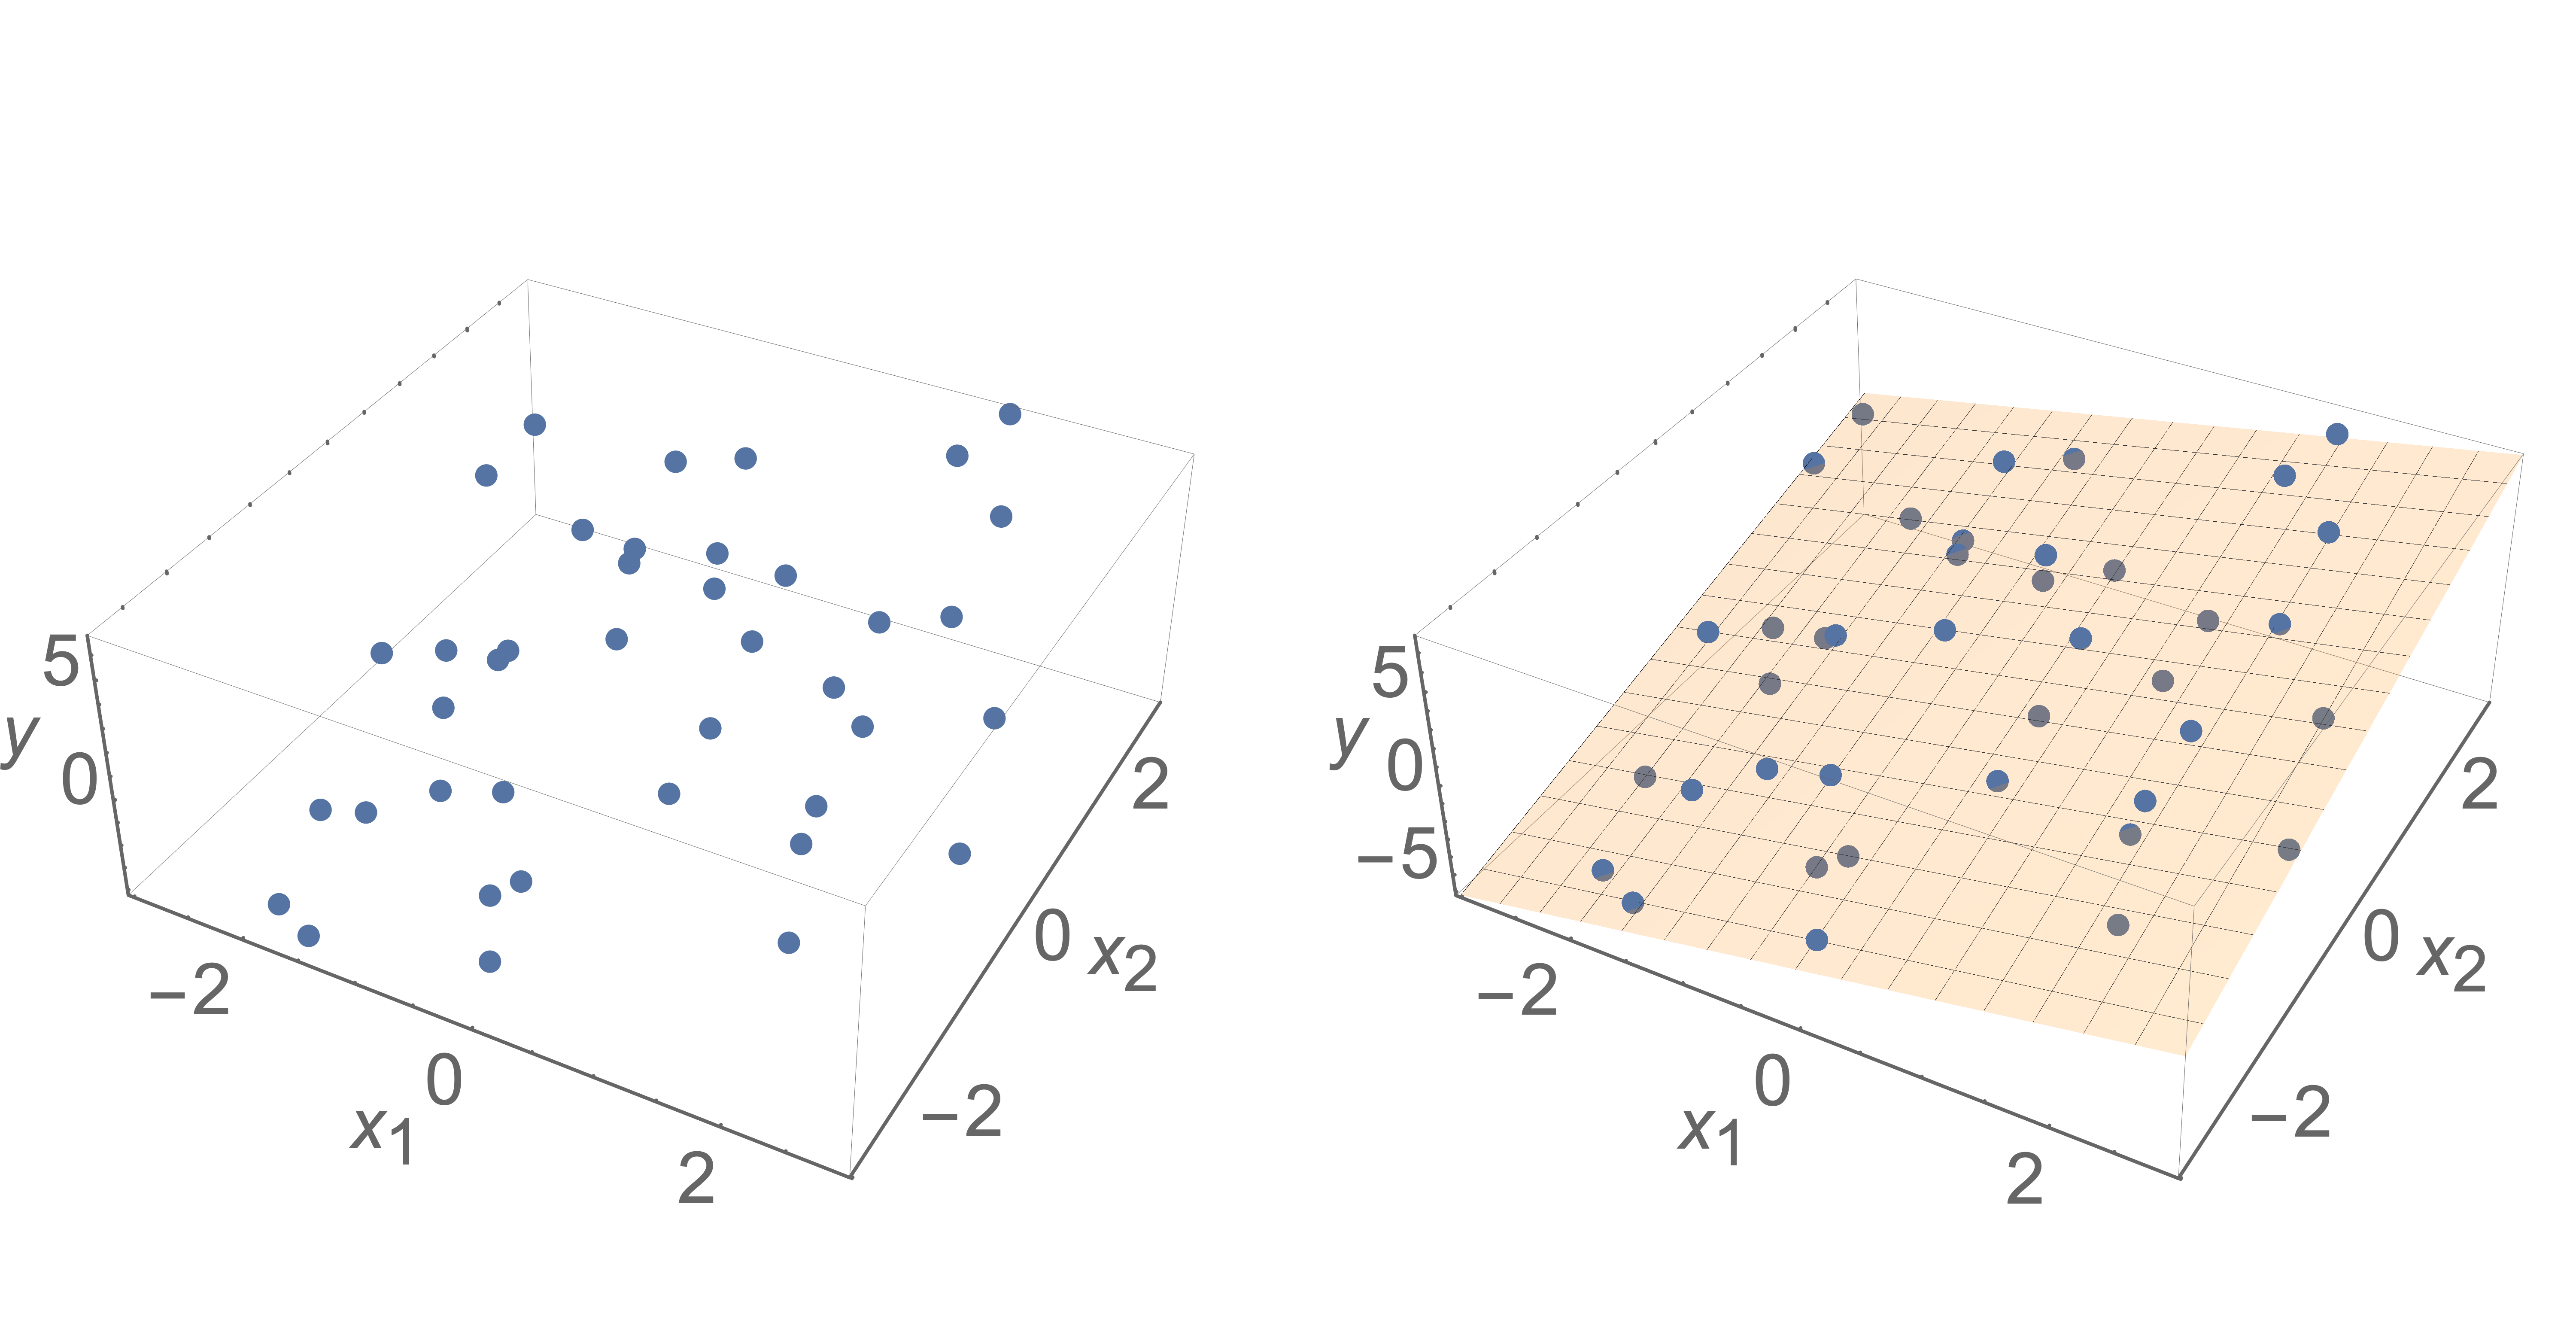
\includegraphics[width=0.9\textwidth]{figures/regression_ex1_plane1.png}

A richer class of hypotheses can be obtained by performing a
non-linear feature transformation before doing the regression, as
we will later see (in Chapter~\ref{chap-features}), but it will still
end up that we have to solve a linear regression problem.

% Here, we begin with the foundations, studying {\em linear} regression, including
% its framing as an optimization problem (Section~\ref{sec-reg_optim}),
% how to use {\em regularization} to keep solutions generalizable
% (Section~\ref{sec-regularization}), and how to evaluate {\em
%   learning algorithms} which solve the regression problem
% (Section~\ref{sec-reg_learn_alg}).


\section{A gloriously simple linear regression algorithm}

Okay!  Given the objective in Eq.~\ref{eq:reg_mse_withconst}, how
can we find good values of $\theta$ and $\theta_0$?  We'll study
several general-purpose, efficient, interesting algorithms.  But
before we do that, let's start with the simplest one we can think of:
{\em guess a whole bunch ($k$) of different values of $\theta$ and
$\theta_0$}, see which one has the smallest error on the training
set, and return it.

\begin{codebox}
  \Procname{$\proc{Random-Regression}(\data, k)$}
  \li For $i$ in  $1\dots k$: Randomly generate hypothesis $\ex{\theta}{i},
    \ex{\theta_0}{i}$
  \li Let $i = \argmin{i} J(\ex{\theta}{i}, \ex{\theta_0}{i}; \data)$
  \li Return $\ex{\theta}{i}, \ex{\theta_0}{i}$
\end{codebox}

This seems kind of silly, but it's a learning algorithm, and it's not
completely useless. \index{regression!random regression}
\question{If your data set has $n$ data points, and the dimension of the
  $x$ values is $d$, what is the size of an individual $\ex{\theta}{i}$?}
\question{How do you think increasing the number of guesses $k$ will change the training
  error of the resulting hypothesis?}


%%%%%%%%%%%%%%%%%%%%%%%%%%%%%%%%%%%%%%%%
\section{Analytical solution: ordinary least squares}

One very interesting aspect of the problem of finding a linear hypothesis
that minimizes mean squared error is that we can find a
closed-form formula for the answer!\note{What does ``closed form''
  mean?  Generally, that it involves direct evaluation of a
  mathematical expression using a fixed number of ``typical''
  operations (like arithmetic operations, trig functions, powers,
  etc.).  So equation~\ref{olsObjective} is not in closed form,
  because it's not at all clear what operations one needs to perform
  to find the solution.} This general problem is often
called the {\em ordinary least squares} ({\sc ols})

Everything is easier to deal with if we assume that all of the the $\ex{x}{i}$
have been augmented with an extra input dimension (feature) that
always has value 1, so that they are in $d+1$ dimensions, and rather
than having an explicit $\theta_0$, we let it be the last element of
our $\theta$ vector, so that we have, simply,
\[y = \theta^T x\;\;.\]
In this case, the objective becomes
\begin{equation}
  J(\theta) = \frac{1}{n}\sum_{i =
    1}^n\left(\theta^Tx^{(i)} - \ex{y}{i}\right)^2 \;\;.
  \label{eq:reg_mse}
\end{equation}

\question{
  Stop and prove to yourself that adding that extra feature
  with value 1 to every input vector and getting rid of the $\theta_0$
  parameter is equivalent to our original model.
}

We approach this just like a minimization problem from calculus
homework:  take the derivative of $J$ with respect to $\theta$, set it
to zero, and solve for $\theta$.  There are additional steps
required, to check that the resulting $\theta$ is a minimum (rather
than a maximum or an inflection point) but we won't work through that
here.   It is possible to approach this problem by:
\begin{itemize}
  \item Finding $\partial{J}/\partial{\theta_k}$ for $k$ in
        \anchorednote{$1, \ldots, d$,}{We will use $d$ here for the total number of features in
          each $\ex{x}{i}$, including the added 1.}
  \item Constructing a set of $k$ equations of the form
        $\partial{J}/\partial{\theta_k} = 0$, and
  \item Solving the system for values of $\theta_k$.
\end{itemize}
That works just fine.  To get practice for applying techniques like
this to more complex problems, we will work through a more compact
(and cool!) matrix view. Along the way, it will be helpful to collect all of the derivatives in one
vector. In particular,
the
gradient of $J$ with respect to $\theta$ is following column vector of length $d$:
\[
  \nabla_\theta J =
  \begin{bmatrix}
    \partial J / \partial \theta_1 \\
    \vdots                         \\
    \partial J / \partial \theta_d
  \end{bmatrix}.
\]

\question{Work through the next steps and check your answer against ours below.}

We can think of our training data in terms of matrices $X$ and $Y$,
where each column of $X$ is an example, and each ``column'' of $Y$ is
the corresponding target output value:
\begin{equation*}
  X = \begin{bmatrix}x_1^{(1)} & \dots & x_1^{(n)} \\\vdots & \ddots &
               \vdots                        \\x_d^{(1)} & \dots & x_d^{(n)}\end{bmatrix} \;\;\;
  Y = \begin{bmatrix}y^{(1)} & \dots & y^{(n)}\end{bmatrix}\;\;.
\end{equation*}
\question{
  What are the dimensions of $X$ and $Y$?
}


In most textbooks, they think of an individual example $\ex{x}{i}$ as
a row, rather than a column.  So that we get an answer that will be
recognizable to you, we are going to define a new matrix and vector,
% $W$ and $T$, which are just transposes of our $X$ and $Y$, and
$\Xt$ and $\Yt$, which are just transposes of our $X$ and $Y$, and
then work with them:
$$ \Xt = X^T = \begin{bmatrix}x_1^{(1)} & \dots & x_d^{(1)}\\\vdots & \ddots & \vdots\\x_1^{(n)} & \dots & x_d^{(n)}\end{bmatrix} \;\;
  \Yt = Y^T = \begin{bmatrix}y^{(1)}\\\vdots\\y^{(n)}\end{bmatrix} \;\;.$$
\question{
  What are the dimensions of $\Xt$ and $\Yt$?
}

Now we can write
\[ J(\theta) = \frac{1}{n}\underbrace{(\Xt\theta - \Yt)^T}_{1 \times
    n}\underbrace{(\Xt\theta - \Yt)}_{n \times 1} =
  \frac{1}{n}\sum_{i=1}^n \left(\left(\sum_{j=1}^d \Xt_{ij}\theta_j
    \right) - \Yt_i\right)^2\]
and using facts about matrix/vector calculus, we get \note{You should
  be able to verify this by doing a simple (say, $2 \times 2$) example by hand.}
\begin{equation}
  \nabla_{\theta}J = \frac{2}{n}\underbrace{\Xt^T}_{d \times n}\underbrace{(\Xt\theta - \Yt)}_{n \times 1}\;\;.
  % \label{eq:reg_gd_deriv}
\end{equation}
See Appendix~\ref{app:matrix_deriv} for a nice way to think about finding this
derivative.

Setting $ \nabla_{\theta}J$ to 0 and solving, we get:
\begin{align*}
  \frac{2}{n}\Xt^T(\Xt\theta - \Yt) & = 0                          \\
  \Xt^T\Xt\theta - \Xt^T \Yt        & = 0                          \\
  \Xt^T\Xt\theta                    & =  \Xt^T \Yt                 \\
  \theta                            & =  (\Xt^T\Xt)^{-1} \Xt^T \Yt \\
\end{align*}
And the dimensions work out!
$$ \theta = \underbrace{\left(\Xt^T\Xt\right)^{-1}}_{d \times d}\underbrace{\Xt^T}_{d \times n}\underbrace{\Yt}_{n \times 1} $$
So, given our data, we can directly compute the linear regression that
minimizes mean squared error.  That's pretty awesome!

%%%%%%%%%%%%%%%%%%%%%%%%%%%%%%%%%%%%%%%%%%%%%%%%%%%%%%%%%%%%%%%%%%%%%%%%%%%%%
\section{Regularization}

\label{sec-regularization}

The objective function of Eq.~\ref{eq:ml_objective_loss} balances
(training-data) memorization, induced by the {\em loss} term, with generalization,
induced by the {\em regularization} term.  Here, we address the need
for regularization specifically for linear regression, and show how
this can be realized using one popular regularization technique called {\em ridge regression}.

%%%%%%%%%%%%%%%%%%%%%%%%%%%%%%%%%%%%%%%%
\subsection{Regularization and linear regression}

If all we cared about was finding a hypothesis with small loss on the
training data, we would have no need for regularization, and could
simply omit the second term in the objective.  But remember that our
ultimate goal is to {\em perform well on input values that we haven't
    trained on!}  It may seem that this is an impossible task, but
humans and machine-learning methods do this successfully all the
time.  What allows {\em generalization} to new input values is a
belief that there is an underlying regularity that governs both the
training and testing data.  One way to
describe an assumption about such a regularity is by choosing a
limited class of possible hypotheses.  Another way to do this is to
provide smoother guidance, saying that, within a hypothesis class, we
prefer some hypotheses to others.  The regularizer articulates this
preference and the constant $\lambda$ says how much we are willing to
trade off loss on the training data versus preference over hypotheses.

%%%%%%%%%%%%%%%%%%%%%%%%%%%%%%%%%%%%%%%%
\begin{comment}
This trade-off is illustrated in the figure below.  Hypothesis $h_1$
has zero training loss, but is very complicated.  Hypothesis $h_2$
mis-classifies two points, but is very simple.  In absence of other
beliefs about the solution, it is often better to prefer that the
solution be ``simpler,'' and so we might prefer $h_2$ over $h_1$,
expecting it to perform better on future examples drawn from this same
distribution.  \note{To establish some vocabulary, we say that
  $h_1$ is {\em overfit} to the training data.}  Another nice way of
thinking about regularization is that we would like to prevent our
hypothesis from being too dependent on the particular training data
that we were given: we would like for it to be the case that if the
training data were changed slightly, the hypothesis would not change
by much.

\begin{center}
  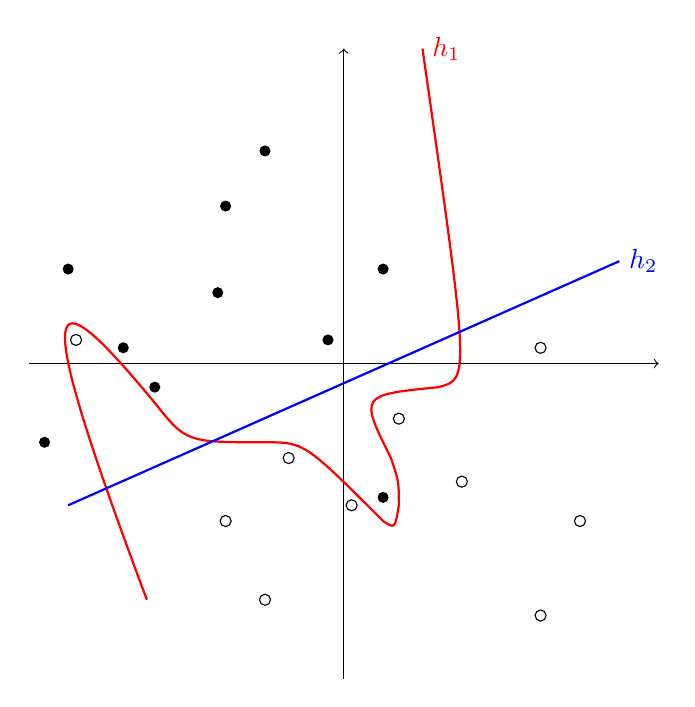
\begin{tikzpicture}
    \draw [->] (-4,0) -- (4,0);
    \draw [->] (0,-4) -- (0,4);
    \draw[red,thick] (-2.5,-3) .. controls (-4,1) and (-3.8,1.2) .. (-2.4,-.5)
    .. controls (-2,-1) .. (-1,-1) .. controls (-.5,-1) ..  (.5,-2)
    .. controls (.65, -2.1) .. (.7,-1.8) .. controls (.7,-1.5)
    ..  (.6,-1.2) .. controls (.2,-.4) .. (1.2, -.3)
    .. controls (1.6,-.2) .. (1,4);

    \foreach \Point in {(-3.4, .3), (2.5, .2), (-1.5,-2), (-1,-3),(.7,-.7),
        (3, -2), (2.5, -3.2), (-.7,-1.2), (0.1,-1.8), (1.5, -1.5)}{
        \draw \Point circle[radius=2pt];
      }
    \foreach \Point in {(.5,-1.7),(-.2,.3),(-2.8,.2),(-2.4,-.3),(-1,2.7),
        (-1.5, 2), (-1.6, .9), (-3.8,-1), (-3.5,1.2),(.5, 1.2)}{
        \fill \Point circle[radius=2pt];
      }
    \draw[blue, thick] (-3.5,-1.8) -- (3.5,1.3);
    \node[right,blue] at (3.5,1.3) {$h_2$};
    \node[below,right,red] at (1,4) {$h_1$};

  \end{tikzpicture}
\end{center}
\end{comment}
%%%%%%%%%%%%%%%%%%%%%%%%%%%%%%%%%%%%%%%%

For example, consider what happens when $d=2,$ and $x_2$ is highly
correlated with $x_1$, meaning that the data look like a line, as
shown in the left panel of the figure below.  Thus, there isn't a \anchorednote{unique best hyperplane}{Sometimes there's technically a
  unique best hyperplane, but just because of noise.}.  Such
correlations happen often in real-life data, because of underlying
common causes; for example, across a population, the height of people
may depend on both age and amount of food intake in the same way.
This is especially the case when there are many feature dimensions
used in the regression.  Mathematically, this leads to $\Xt^T\Xt$
close to singularity, such that $(\Xt^T\Xt)^{-1}$ is undefined or has huge
values, resulting in unstable models (see the middle panel of figure
and note the range of the $y$ values---the slope is huge!):

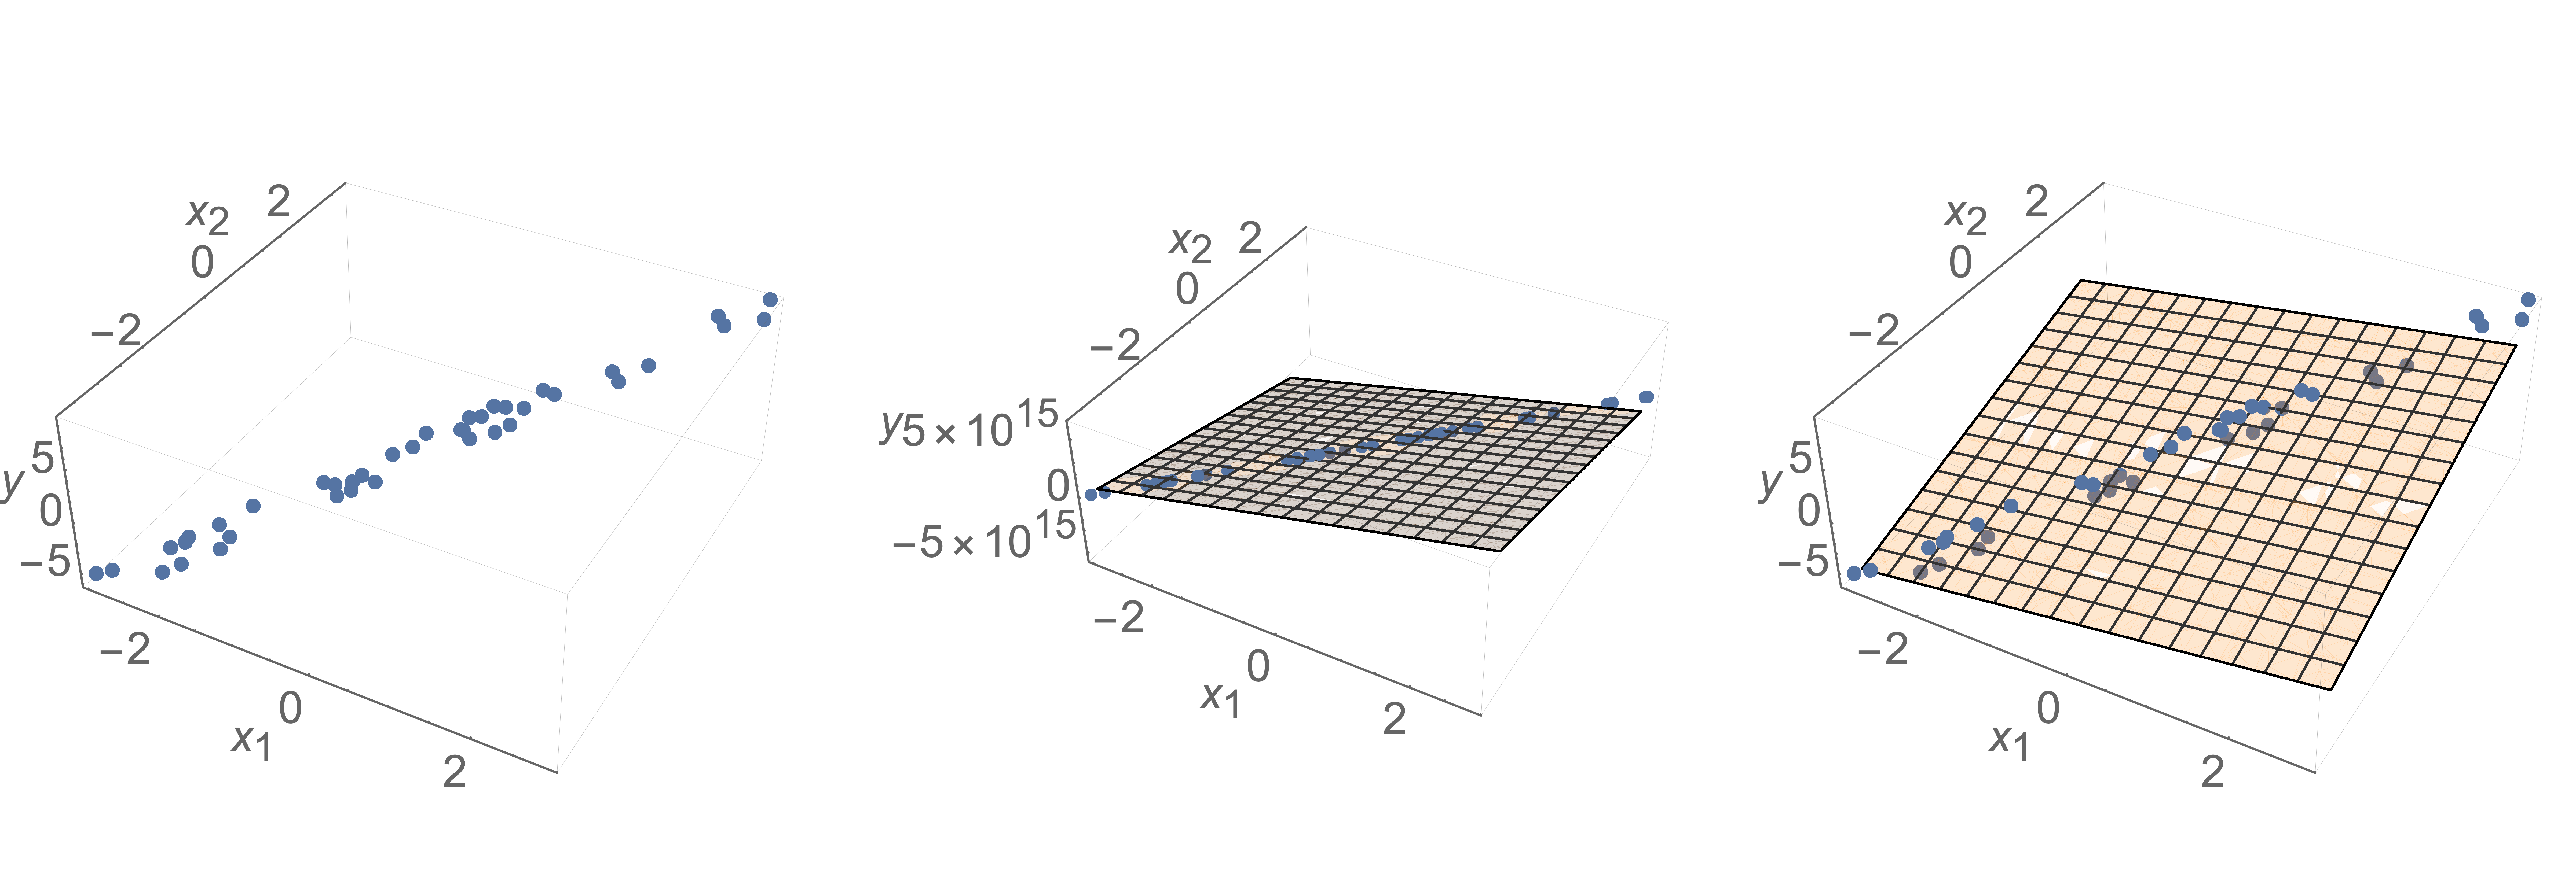
\includegraphics[width=1.12\textwidth]{figures/regression_ex2_plane1.png}

% (* mathematica: effect of regularization *)
% npts = 40;
% SeedRandom[3];
% x1 = RandomReal[{-3, 3}, {npts}];
% x2 = 1.2 * x1 + 0.3;
% noise = RandomReal[{-1.5, 1.5}, {npts}];
% yv = x1 + 1.4 * x2 + 1 + noise;
% pts = Transpose@{x1, x2, yv};
%
% regmodel =
%  Fit[pts, {1, Subscript[x, 1], Subscript[x, 2]}, {Subscript[x, 1],
%    Subscript[x, 2]}, FitRegularization -> {Tikhonov, 0.1}]
%
% model =
%  LinearModelFit[
%   pts, { Subscript[x, 1], Subscript[x, 2]}, { Subscript[x, 1],
%    Subscript[x, 2]}]
%
% p1 = ListPointPlot3D[ pts,
%    AxesLabel -> {Subscript[x, 1], Subscript[x, 2], y} ];
% p2 = ListPlot3D[ pts ];
% p3 = Plot3D[
%    model[Subscript[x, 1], Subscript[x, 2]], {Subscript[x, 1], -3,
%     3}, {Subscript[x, 2], -3, 3}, PlotStyle -> Opacity[0.2]
%    ];
% p5 = Plot3D[
%    regmodel, {Subscript[x, 1], -3, 3}, {Subscript[x, 2], -3, 3},
%    PlotStyle -> Opacity[0.2]];
% p4 = Show[{p1, p3}];
% p6 = Show[{p1, p5}];
% gr1 = GraphicsRow[{p1, p4, p6}, ImageSize -> Large]
% Export["regression_ex2_plane1.png", gr1, ImageResolution -> 1200]

A common strategy for specifying a \emph{regularizer} is to use the form
\[ R(\Theta) = \norm{\Theta - \Theta_{\it prior}}^2 \]
when we have some idea in advance that $\Theta$ ought to be near some
value $\Theta_{\it prior}$.
\note{Learn about Bayesian methods in machine learning to see the theory behind this and cool results!}

Here, the notion of distance is quantified by squaring the $l_2$ \textit{norm} of
the parameter vector: for any $d$-dimensional vector $v \in \mathbb{R}^d,$ the $l_2$ \textit{norm} of $v$ is defined as,
\[\|v\| = \sqrt{\sum_{i=1}^d |v_i|^2}\;\;. \]
In the absence of such knowledge a default is
to {\em regularize toward zero}:
\[ R(\Theta) = \norm{\Theta}^2\;\;. \]
%
When this is done in the example depicted above, the regression model
becomes stable, producing the result shown in the right-hand panel in
the figure.  Now the slope is much more sensible.


%%%%%%%%%%%%%%%%%%%%%%%%%%%%%%%%%%%%%%%%
\subsection{Ridge regression}

\label{sec-ridge_regression}

There are some kinds of trouble we can get into in regression problems.
What if $\left(\Xt^T\Xt\right)$ is not invertible?
\question{Consider, for example, a situation where the data-set is
just the same point repeated twice:
$\ex{x}{1} = \ex{x}{2} = [1~~2]^T$.
What is $\Xt$ in this case?  What is $\Xt^T\Xt$?  What is $(\Xt^T\Xt)^{-1}$?
}

Another kind of problem is {\em overfitting}: we have formulated an
objective that is just about fitting the data as well as possible, but
we might also
want to {\em regularize} to keep the hypothesis from getting {\em too}
attached to the data.

We address both the problem of not being able to invert $(\Xt^T\Xt)^{-1}$ and
the problem of overfitting using a mechanism called {\em ridge
    regression}.  We add a regularization term $\|\theta\|^2$ to the
  {\sc ols} objective, with a non-negative scalar value $\lambda$ to control the tradeoff
between the training error and the regularization term.
\question{Why do we emphasize the non-negativity of the scalar $\lambda?$ When we add a regularizer of the form $\|\theta\|^2$, what
  is our most ``preferred'' value of $\theta$, in the absence of any
  data?}
Here is the ridge regression objective function:\index{regression!ridge regression}
$$ J_{\text{ridge}}(\theta, \theta_0) = \frac{1}{n}\sum_{i = 1}^n\left(\theta^Tx^{(i)} + \theta_0 - y^{(i)}\right)^2 + \lambda\|\theta\|^2 $$
Larger $\lambda$ values pressure $\theta$ values to be near zero.
Note that we don't penalize $\theta_0$; intuitively, $\theta_0$ is
what ``floats'' the regression surface to the right level for the data
you have, and so you shouldn't make it harder to fit a data set where
the $y$ values tend to be around one million than one where they tend
to be around one.  The other parameters control the orientation of the
regression surface, and we prefer it to have a not-too-crazy
orientation.

There is an analytical expression for the $\theta, \theta_0$ values
that minimize $J_\text{ridge}$, but it's a little bit more complicated
to derive than the solution for {\sc ols} because $\theta_0$ needs
special treatment.   If we decide not to treat $\theta_0$ specially
(so we add a 1 feature to our input vectors as discussed above), then we get:
$$ \nabla_{\theta}J_\text{ridge} = \frac{2}{n}\Xt^T(\Xt\theta - \Yt) + 2
  \lambda \theta\;\;.$$

Setting to 0 and solving, we get:\note{Remember that $I$ stands for
  the identity matrix, a square matrix that has 1's along the diagonal and 0's
  everywhere else.}
\begin{align*}
  \frac{2}{n}\Xt^T(\Xt\theta - \Yt) + 2 \lambda \theta             & = 0                                      \\
  \frac{1}{n}\Xt^T\Xt\theta - \frac{1}{n}\Xt^T\Yt + \lambda \theta & = 0                                      \\
  \frac{1}{n}\Xt^T\Xt\theta  + \lambda \theta                      & = \frac{1}{n}\Xt^T\Yt                    \\
  \Xt^T\Xt\theta  + n \lambda \theta                               & = \Xt^T\Yt                               \\
  (\Xt^T\Xt  + n \lambda I)\theta                                  & = \Xt^T\Yt                               \\
  \theta                                                           & = (\Xt^T\Xt  + n \lambda I)^{-1}\Xt^T\Yt
\end{align*}
Whew!  So the solution is:
\begin{equation}
  \theta_{\text{ridge}} = \left(\Xt^T\Xt + n\lambda I\right)^{-1}\Xt^T\Yt
  \label{eq:ridge_regression_solution}
\end{equation}

Now, why is the term $\left(\Xt^T\Xt + n\lambda I\right)$\note{This is called 
``ridge'' regression because we are adding a ``ridge'' of $n\lambda$ 
values along the diagonal of the matrix before inverting it.} invertible? 
Explaining this requires some linear algebra. The matrix $\Xt^T\Xt$ is positive 
semidefinite, which implies that its eigenvalues $\{\gamma_i\}_i$ are greater
than or equal to 0. The matrix $\Xt^T\Xt+n\lambda I$ has eigenvalues 
$\{\gamma_i+n\lambda\}_i$ which are guaranteed to be strictly positive since
$\lambda>0$. Recalling that the determinant of a matrix is simply the product of its eigenvectors, 
we get that $\det(\Xt^T\Xt + n\lambda I)>0$ and conclude that $\Xt^T\Xt + n\lambda I$ is invertible.

\question{Why is $\Xt^T\Xt$ positive semidefinite?}
\question{What is the dimension of $I$ in the equation above?}



%%%%%%%%%%%%%%%%%%%%%%%%%%%%%%%%%%%%%%%%%%%%%%%%%%%%%%%%%%%%%%%%%%%%%%%%%%%%%
\section{Evaluating learning algorithms}\label{sec-reg_learn_alg}

In this section, we will explore how to evaluate supervised
machine-learning algorithms.  We will study the special case of
applying them to regression problems, but the basic ideas of
validation, hyper-parameter selection, and cross-validation apply much
more
broadly.

We have seen how linear regression is a well-formed optimization
problem, which has an analytical solution when ridge regularization is
applied.  But how can one choose the best amount of regularization, as
parameterized by $\lambda$?  Two key ideas involve the evaluation of
the performance of a hypothesis, and a separate evaluation of the
algorithm used to produce hypotheses, as described below.

%%%%%%%%%%%%%%%%%%%%%%%%%%%%%%%%%%%%%%%%
\subsection{Evaluating hypotheses}

The performance of a given hypothesis $h$ may be evaluated by
measuring {\em test error} on data that was not used to
%
\anchorednote{train it.}{It's a bit funny to interpret the analytical
  formulas given above for $\theta$ as ``training,'' but later when we employ more statistical methods
  ``training'' will be a meaningful concept.}
%
Given a training set $\data_n,$ a regression hypothesis $h$, and if we choose squared loss, we can define the OLS {\em{training error}} of $h$ to be the mean square error between its predictions and the expected outputs:
\begin{eqnarray*}
  \trainerr(h) = \frac{1}{n}\sum_{i = 1}^{n} \left[ h(\ex{x}{i}) - \ex{y}{i} \right]^2
  \;\;.
\end{eqnarray*}
Test error captures the performance of $h$ on unseen data, and is the
mean square error on the test set, with a nearly identical expression
as that above, differing only in the range of index $i$:
\begin{eqnarray*}
  \mathcal{E}(h) = \frac{1}{n'}\sum_{i = n + 1}^{n + n'} \left[ h(x^{(i)}) - y^{(i)} \right]^2
\end{eqnarray*}
on $n'$ new examples that were not used in the process of constructing $h$.

In machine learning in general, not just regression, it is useful to
distinguish two ways in which a hypothesis $h \in \hclass$ might
contribute to test error. Two are:
\begin{description}
  \item{\bf Structural error}: This is error that arises because there
        is no hypothesis $h \in \hclass$ that will perform well on the data,
        for example because the data was really generated by a sine wave but
        we are trying to fit it with a line.\index{structural error}
  \item{\bf Estimation  error}:  This is error that arises because we
        do not have enough data (or the data are in some way unhelpful) to
        allow us to choose a good $h \in \hclass$, or because we didn't
        solve the optimization problem well enough to find the best $h$
        given the data that we had.\index{estimation error}
\end{description}

\note{There are technical definitions of these concepts that are
  studied in more advanced treatments of machine learning.  Structural
  error is referred to as {\em bias} and estimation error is referred
  to as {\em variance}.}
When we increase $\lambda$, we tend to increase structural error  but
decrease estimation error, and vice versa.

% \question{
% Consider using a polynomial basis of order $k$ as a feature
% transformation $\phi$ on your data.  Would increasing $k$ tend to
% increase or decrease structural error?  What about estimation error?
% }

%%%%%%%%%%%%%%%%%%%%%%%%%%%%%%%%%%%%%%%%
\subsection{Evaluating learning algorithms}

{\em Note that this section is relevant to learning algorithms
  generally---we are just introducing the topic here since we now have
  an algorithm that can be evaluated!}

\vskip0.2in

A {\em learning algorithm}\index{learning algorithm} is a procedure that takes a data set
$\data_n$ as input and returns an hypothesis $h$ from a hypothesis
class $\hclass$; it looks like
\begin{equation*}
  \data_n \longrightarrow \boxed{\text{learning alg ($\hclass$)}} \longrightarrow h
\end{equation*}
%
% $\theta$ and $\theta_{0}$.
Keep in mind that $h$ has parameters. The learning algorithm itself may have its own parameters, and such
parameters are often called {\em hyperparameters}.  The analytical
solutions presented above for linear regression,
e.g., Eq.~\ref{eq:ridge_regression_solution}, may be thought of as
learning algorithms, where $\lambda$ is a hyperparameter that governs
how the learning algorithm works and can strongly affect its performance.

How should we evaluate the performance of a {learning algorithm}?
This can be tricky.  There are many potential sources of variability in
the possible result of computing test error on a learned hypothesis $h$:
\begin{itemize}
  \item Which particular {\em training examples} occurred in $\dataTrain$
  \item Which particular {\em testing examples} occurred in $\dataTest$
  \item Randomization inside the learning {\em algorithm} itself
\end{itemize}

\subsubsection{Validation}
Generally, to evaluate how well a learning {\em algorithm} works,
given an unlimited data source,
we would like to execute the following process multiple
times:
\begin{itemize}
  \item Train on a new training set (subset of our big data source)
  \item Evaluate resulting $h$ on a {\em validation set} that does not
        overlap the training set (but is still a subset of our same big
        data source)
\end{itemize}
% Average the performance of the resulting hypotheses over the different
% ``trials'' of training and validation.

Running the algorithm multiple times controls for possible poor choices of
training set or unfortunate randomization inside the algorithm itself.

\subsubsection{Cross validation}
\label{cross-validation}
One concern is that we might need a lot of data to do this, and in
many applications data is expensive or difficult to acquire. We can
re-use data with {\em{cross validation}}\index{cross validation} (but it's harder to do theoretical
analysis).  \\
\begin{codebox}
  \Procname{$\proc{Cross-Validate}(\data, k)$}
  \li divide $\data$ into $k$ chunks $\data_1, \data_2, \ldots \data_k$ (of roughly equal size)
  \li \For $i \gets 1$ \To $k$
  \li   \Do
  train $h_i$ on $\data \setminus \data_i$ (withholding chunk $\data_i$ as the validation set)
  \li     compute ``test'' error $\mathcal{E}_i (h_i)$ on withheld data $\data_i$
  \End
  \li \Return $\frac{1}{k} \sum_{i=1}^k \mathcal{E}_i (h_i)$
\end{codebox}

It's very important to understand that (cross-)validation neither
delivers nor evaluates a single particular hypothesis $h$.  It
evaluates the {\em learning algorithm} that produces hypotheses.

\subsubsection{Hyperparameter tuning}
The hyper-parameters of a learning algorithm affect how the algorithm
  {\em works} but they are not part of the resulting hypothesis.  So,
for example, $\lambda$ in ridge regression affects {\em which}
hypothesis will be returned, but $\lambda$ itself doesn't show up in
the hypothesis (the hypothesis is specified using parameters $\theta$ and
$\theta_0$).

You can think about each different setting of a hyper-parameter as
specifying a different learning algorithm.

In order to pick a good value of the hyper-parameter, we often end up
just trying a lot of values and seeing which one works best via
validation or cross-validation.\index{hyperparameter!hyperparameter tuning}


\question{How could you use cross-validation to decide whether to use
  analytic ridge regression or our random-regression algorithm and to pick
  $K$ for random regression or $\lambda$ for ridge regression?}



%%% Local Variables:
%%% mode: latex
%%% TeX-master: "top"
%%% End:
